\documentclass{article}
\usepackage{vmargin}
\usepackage{amsmath}
\usepackage{graphicx}
\usepackage{listings}
\usepackage{moreverb}
\usepackage{indentfirst}
\usepackage{url}
\usepackage{float}
\setmarginsrb{1in}{0.5in}{1in}{0.2in}{12pt}{11mm}{0pt}{11mm}
\begin{document}
	\begin{center}
		{\bf \Large Duke 250/16 Processor Core Design}
	\end{center}
	\section{Overview}
	The processor design has followed the Duke 250/16 ISA specification and successfully implemented all of the following instructions.
	\begin{figure}[H]
		\begin{center}
			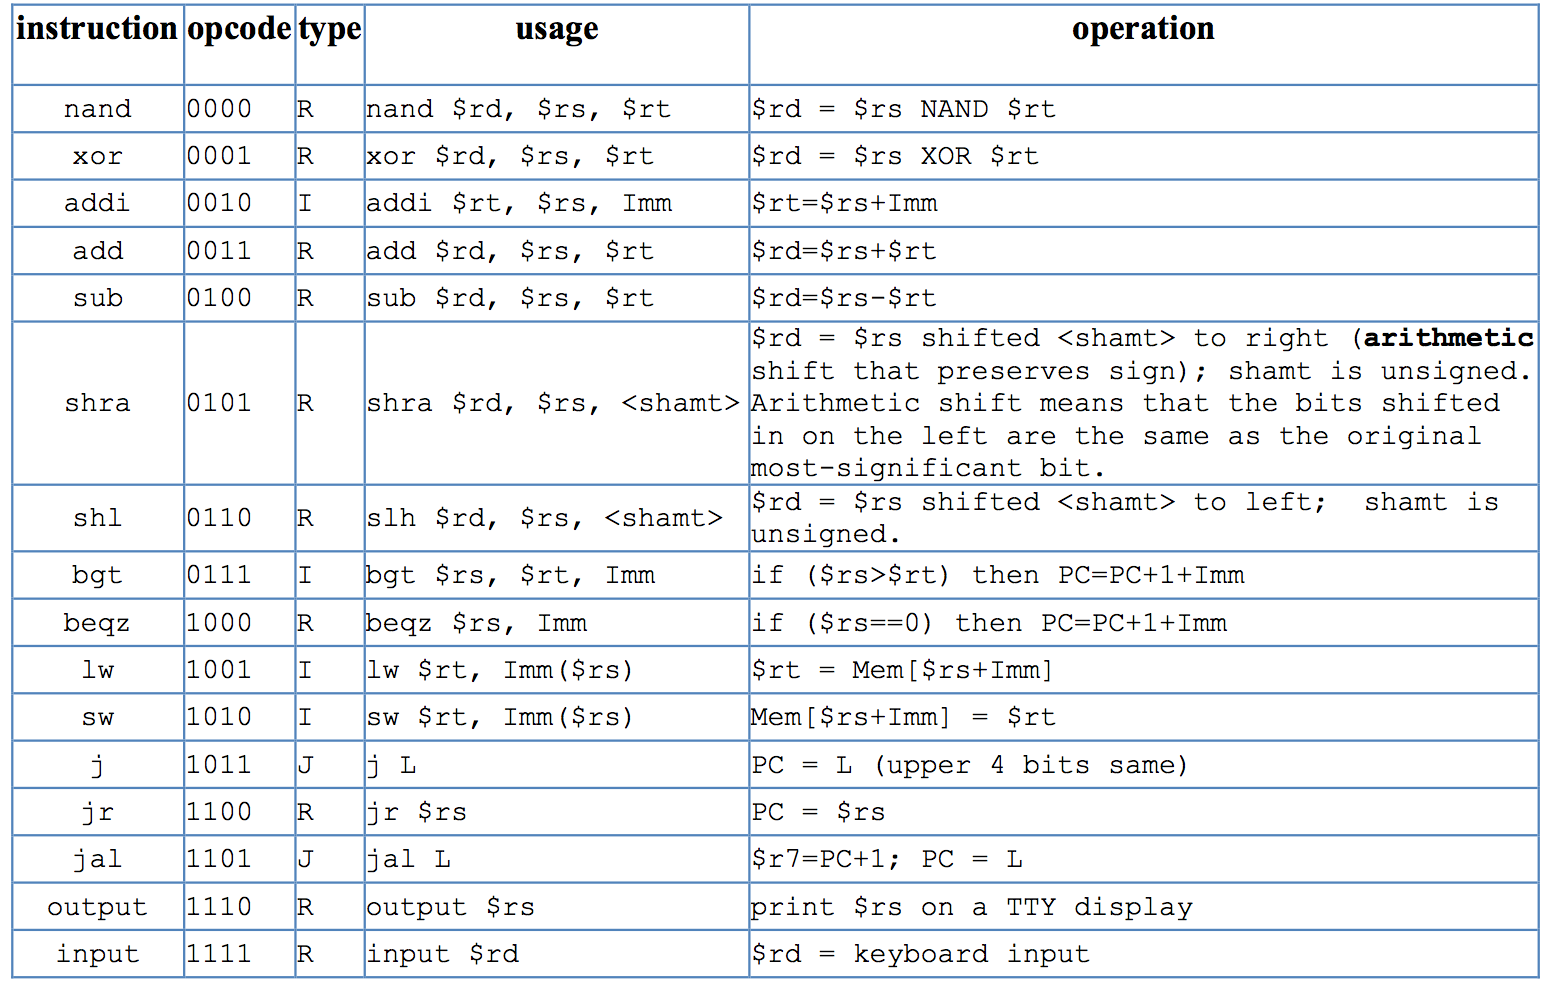
\includegraphics[scale=0.5]{ins}
			\caption{Table of Instructions Implemented}
		\end{center}
	\end{figure}
	\clearpage
	Below is an overview of the main interface of the processor core:
	\begin{figure}[H]
		\begin{center}
			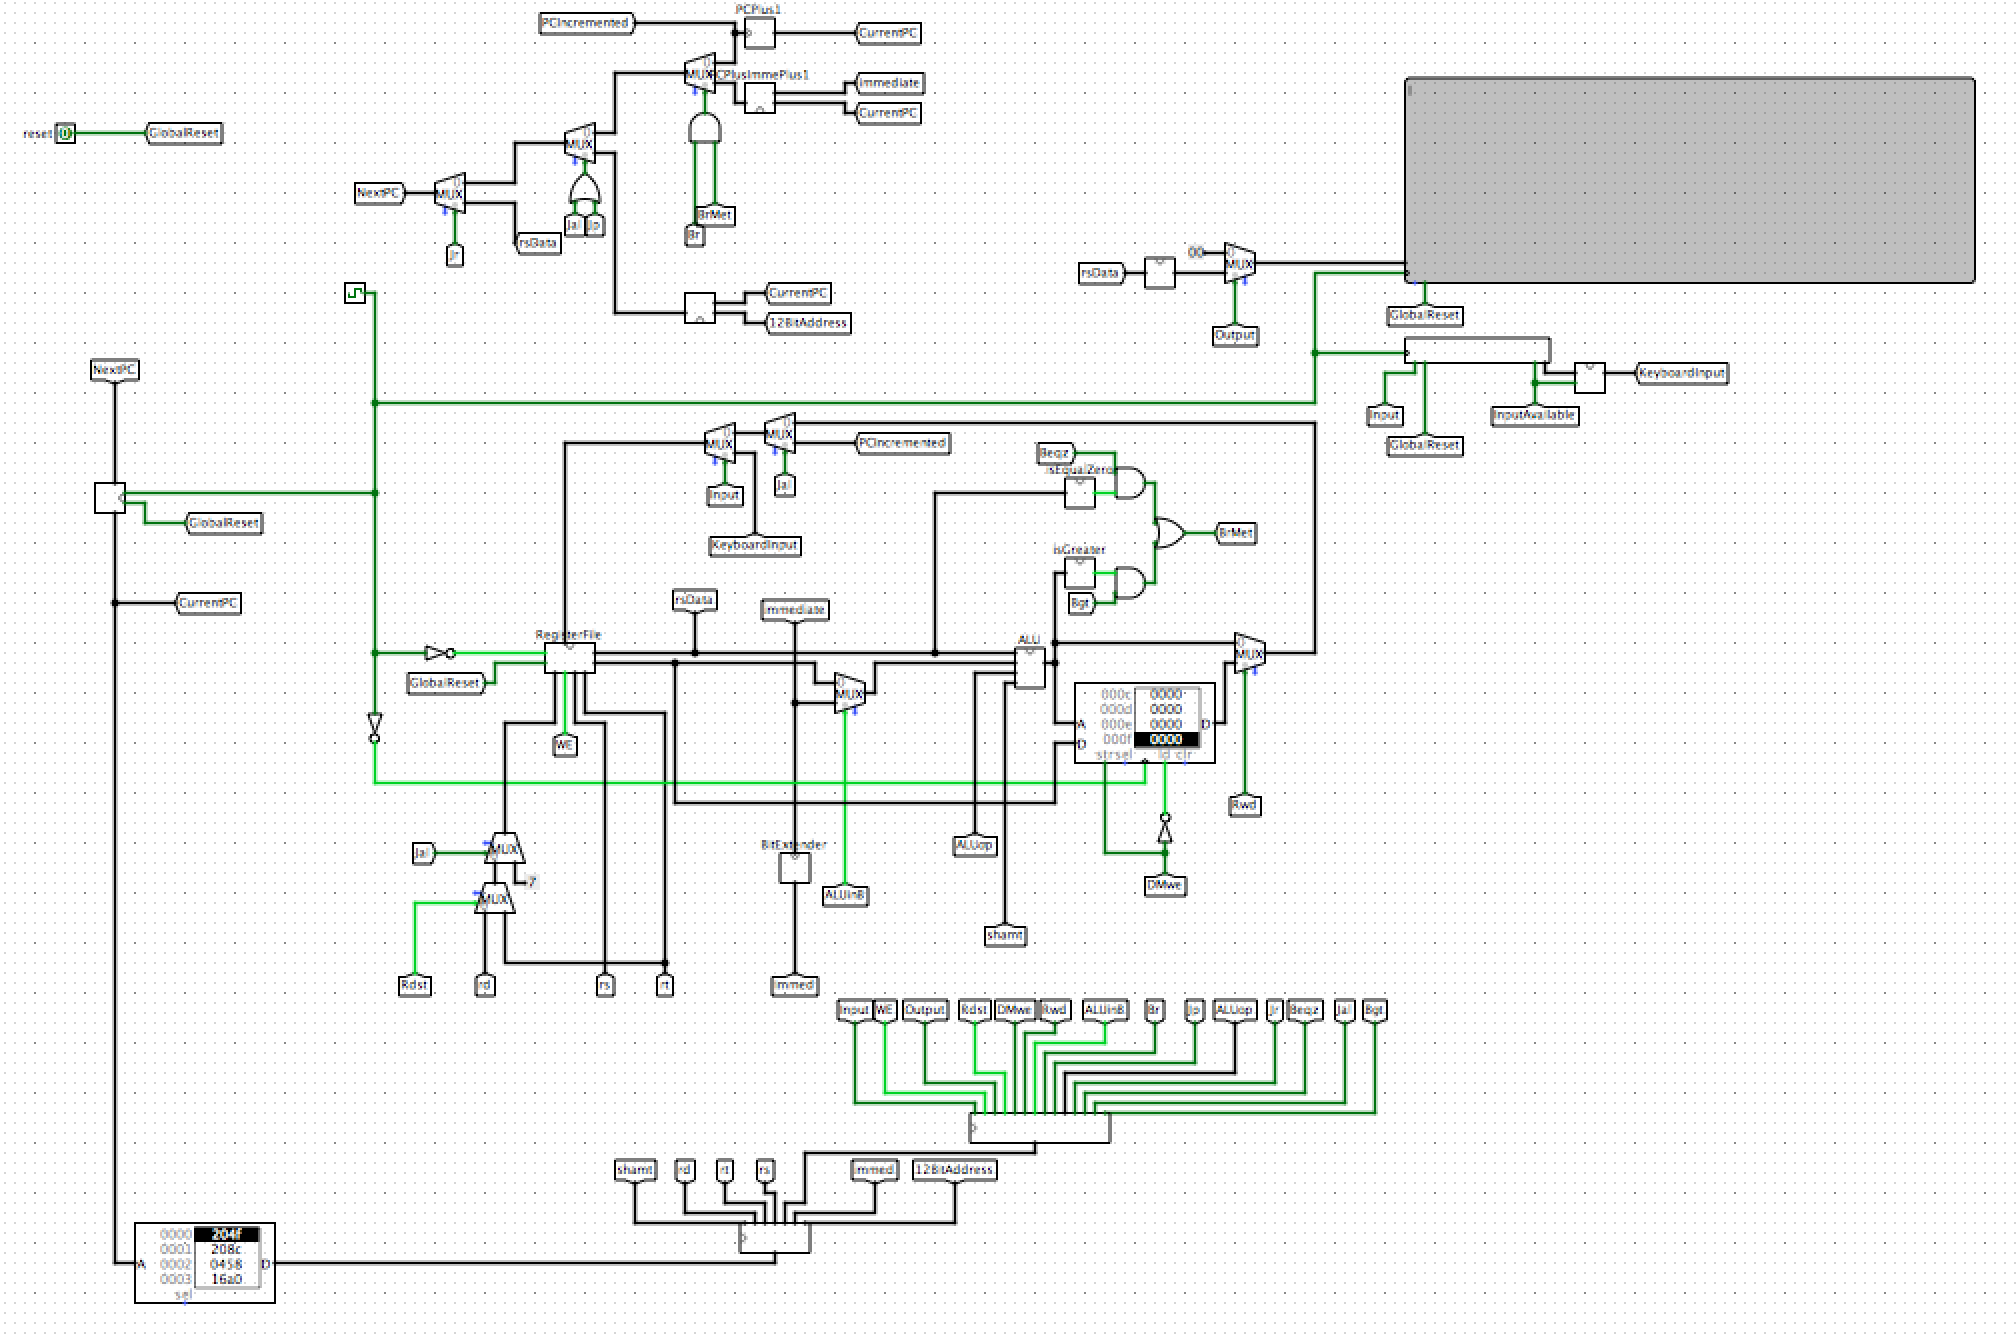
\includegraphics[scale=0.5]{cpu}
			\caption{Integrated View of the Processor Core}
		\end{center}
	\end{figure}
	The processor core has a few major components, the keyboard input, the tty display, the PC register, the instruction ROM, the data memory, the register file, the ALU and the control logic.
	\clearpage
	\section{Register File}
	\begin{figure}[H]
		\begin{center}
			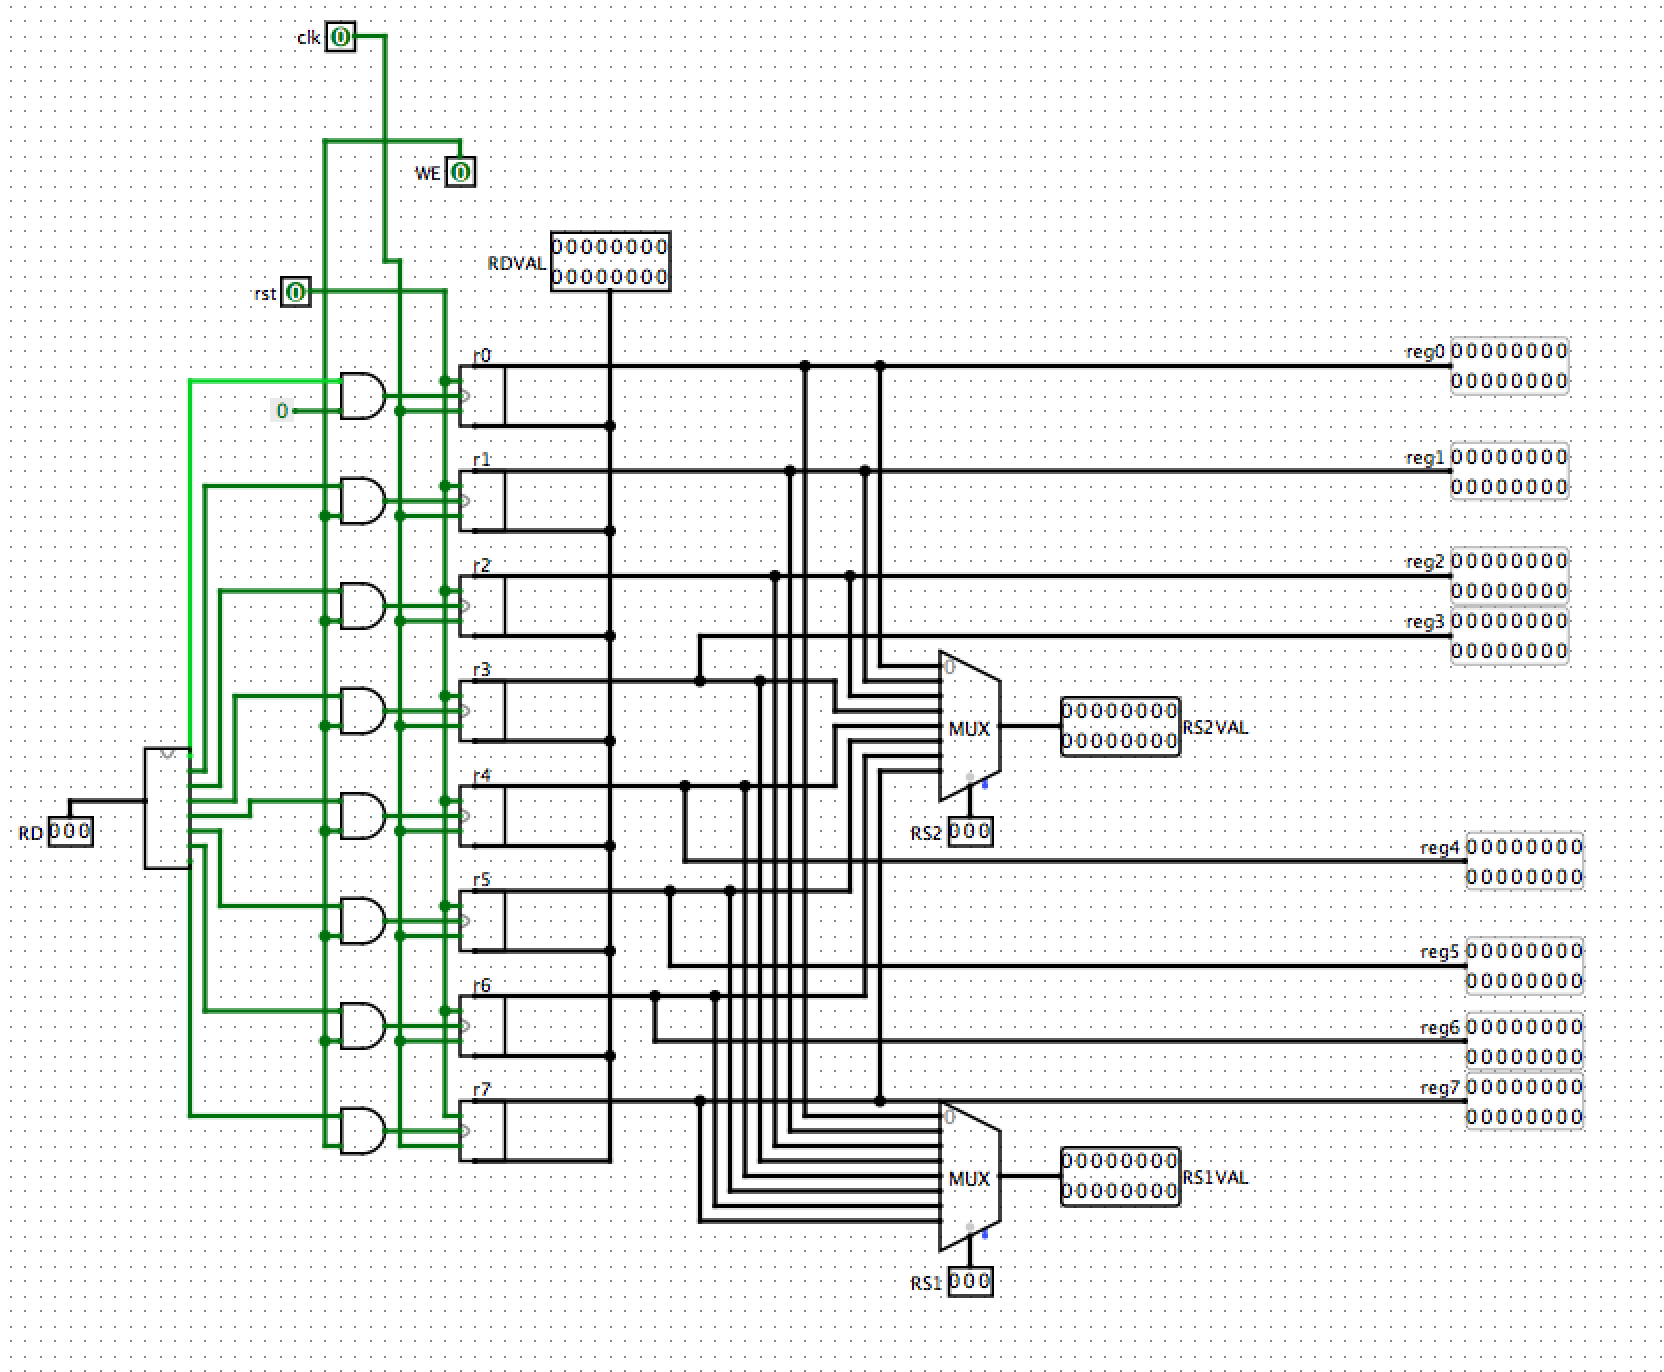
\includegraphics[scale=0.5]{regfile}
			\caption{Register File}
		\end{center}
	\end{figure}
	The register file consists of 7 general purpose registers and a zero register. The interface provides two parallel data reading ports which are labeled as RS1, RS1VAL and RS2, RS2VAL. A three-bit binary input to RS1 and RS2 are required to indicate the register to read and register data will be output through the corresponding output pin. The register file also provides a single write port, and RD input is used to designate the register to write the data input in RDVAL. On top of the IO interface, there are also two more inputs which are the clock pin and global reset pin. 
	\clearpage
	\section{ALU}
	\begin{figure}[H]
		\begin{center}
			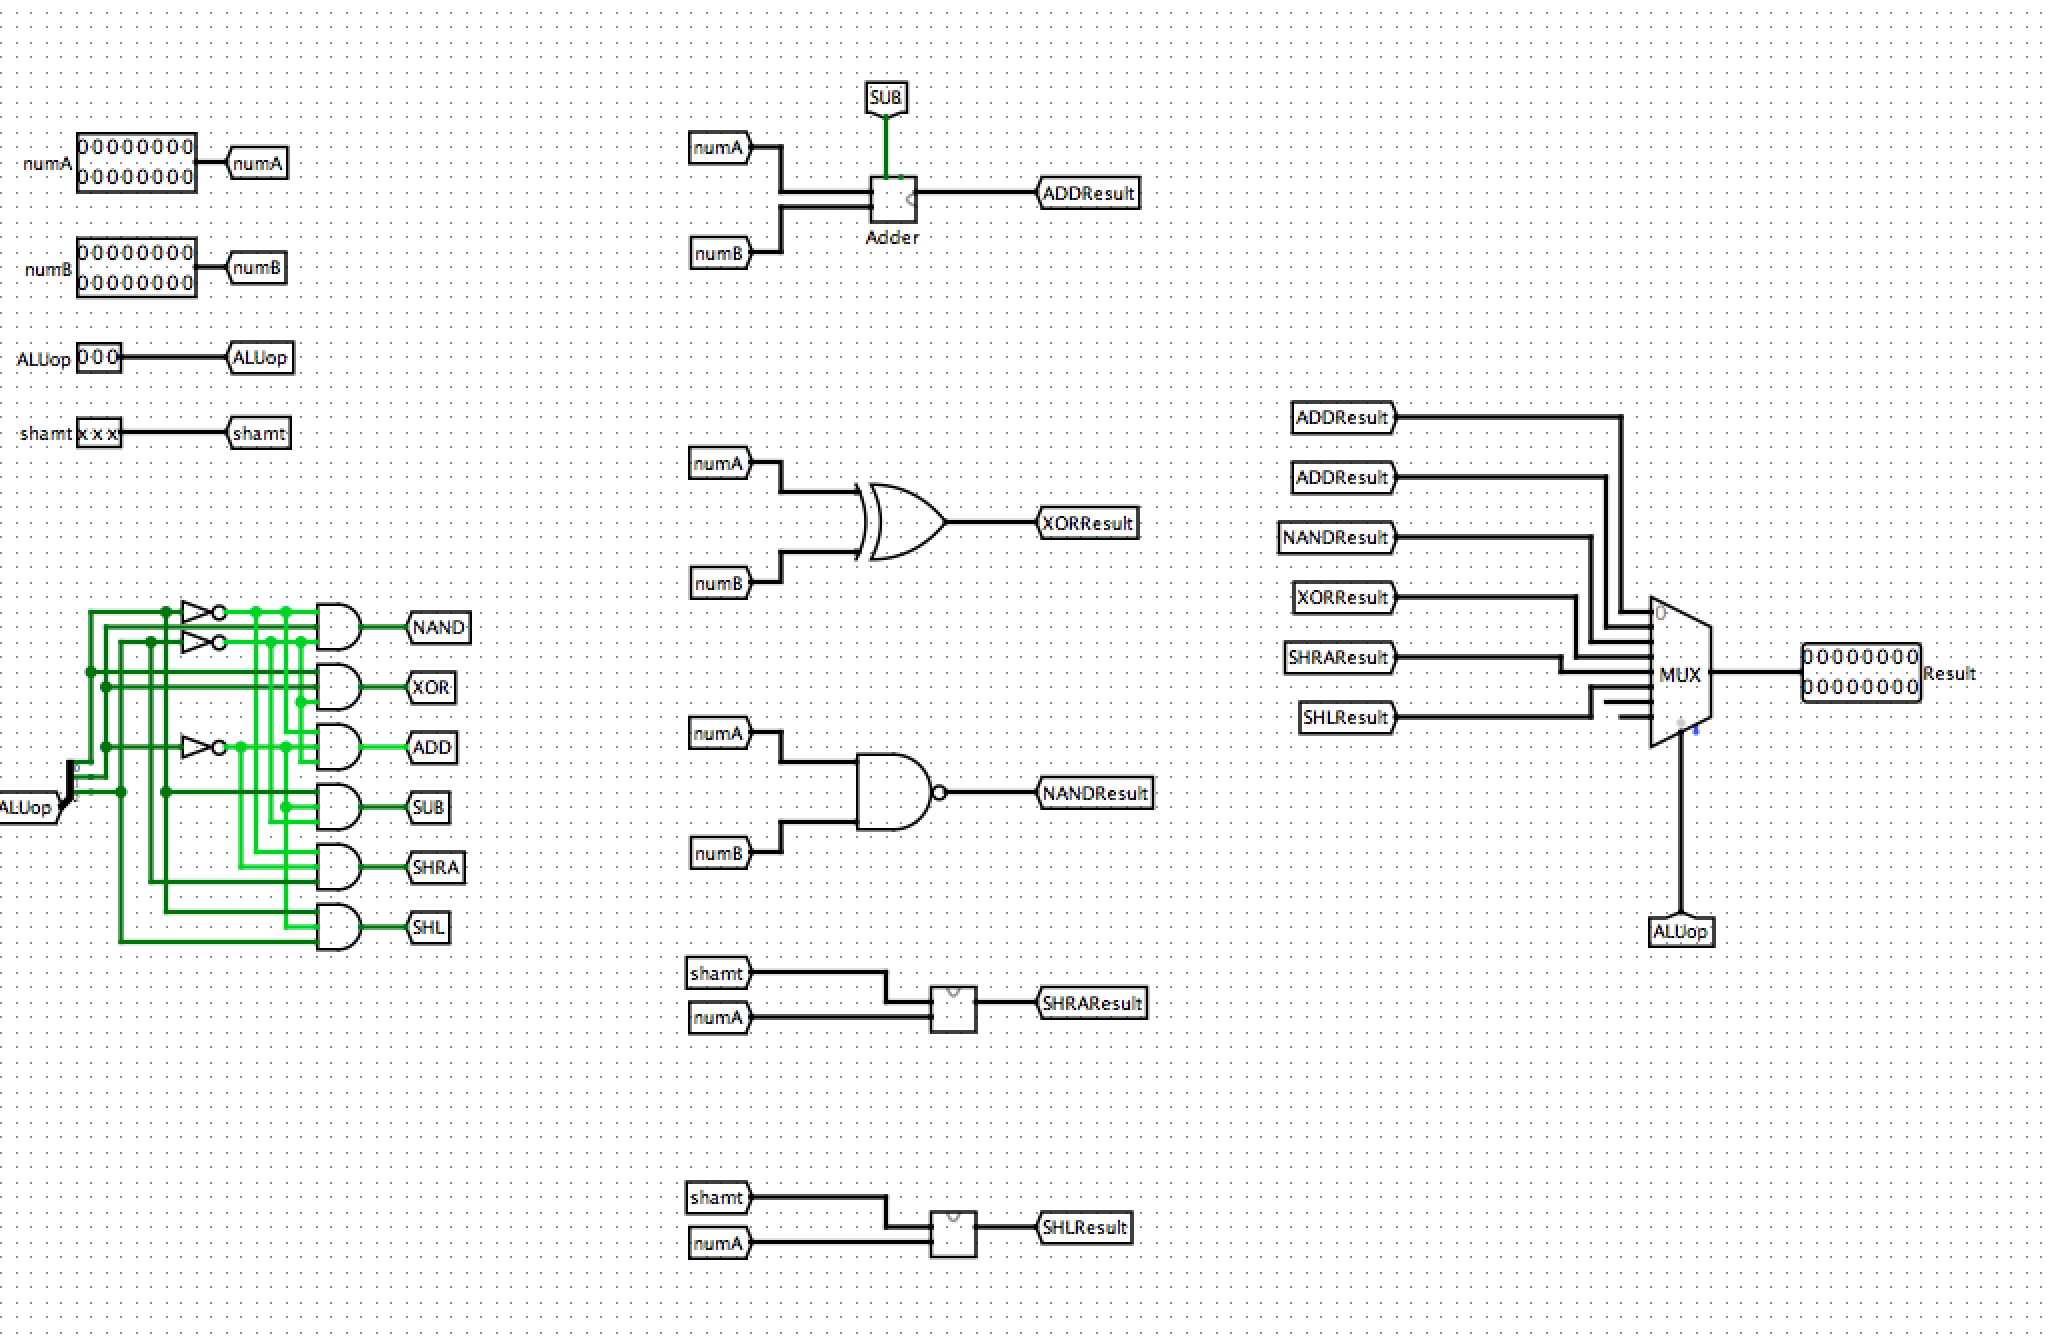
\includegraphics[scale=0.5]{alu}
			\caption{ALU Implementation}
		\end{center}
	\end{figure}
	There are two data inputs to the ALU, denoted as numA and numB. These two numbers represent the operands. shamt is the special three-bit input to the ALU if the ALU is to perform binary shift. It denotes the number of bits to be shifted left or right. Finally it is the three-bit ALUop. ALUop is used to signify which arithmetic operation is required. The supported operations are NAND (010), XOR(011), ADD(000), SUB(001), SHRA(100), SHL(101).
	\clearpage
	\section{PC Register}
	\begin{figure}[H]
		\begin{center}
			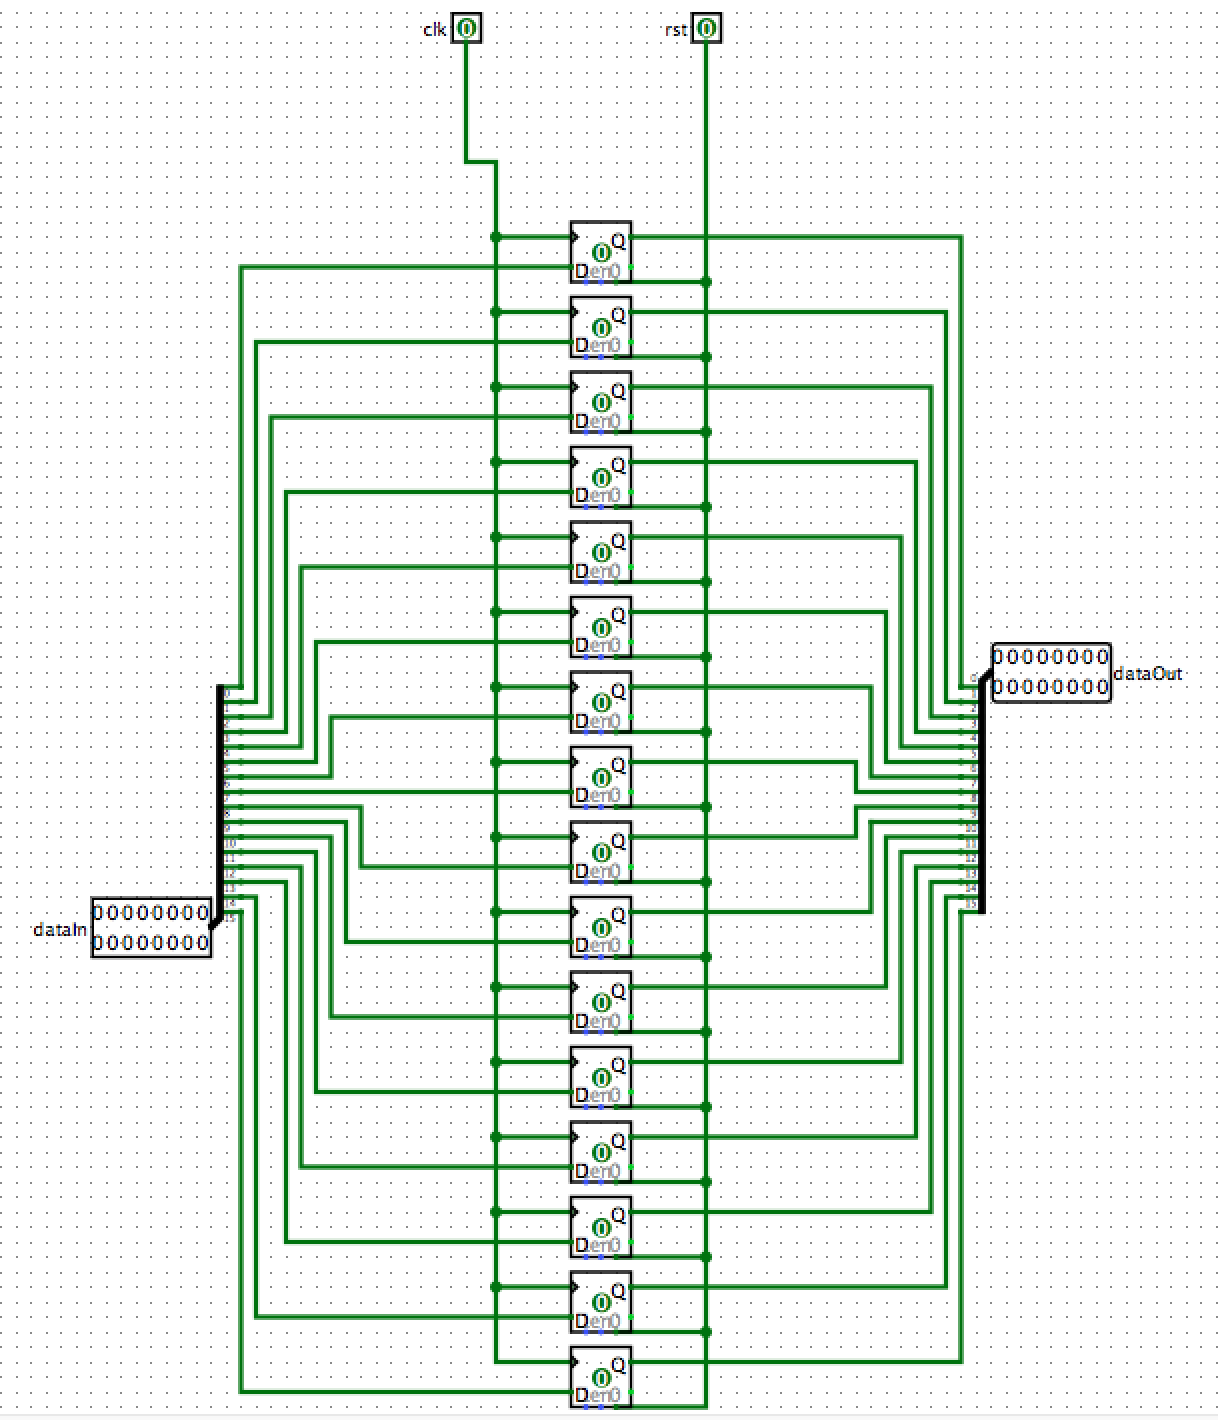
\includegraphics[scale=0.5]{pc}
			\caption{PC Register}
		\end{center}
	\end{figure}
	Just like the general purpose registers, the PC register is implemented using 16 D flip-flops set to trigger at the rising edge. Other than the global reset and clock input, it also has dataIn input and dataOut output ports. dataOut outputs the current PC register value and dataIn gives the new PC value to be stored in the PC register. 
	\clearpage
	\section{Decoder}
	\begin{figure}[H]
		\begin{center}
			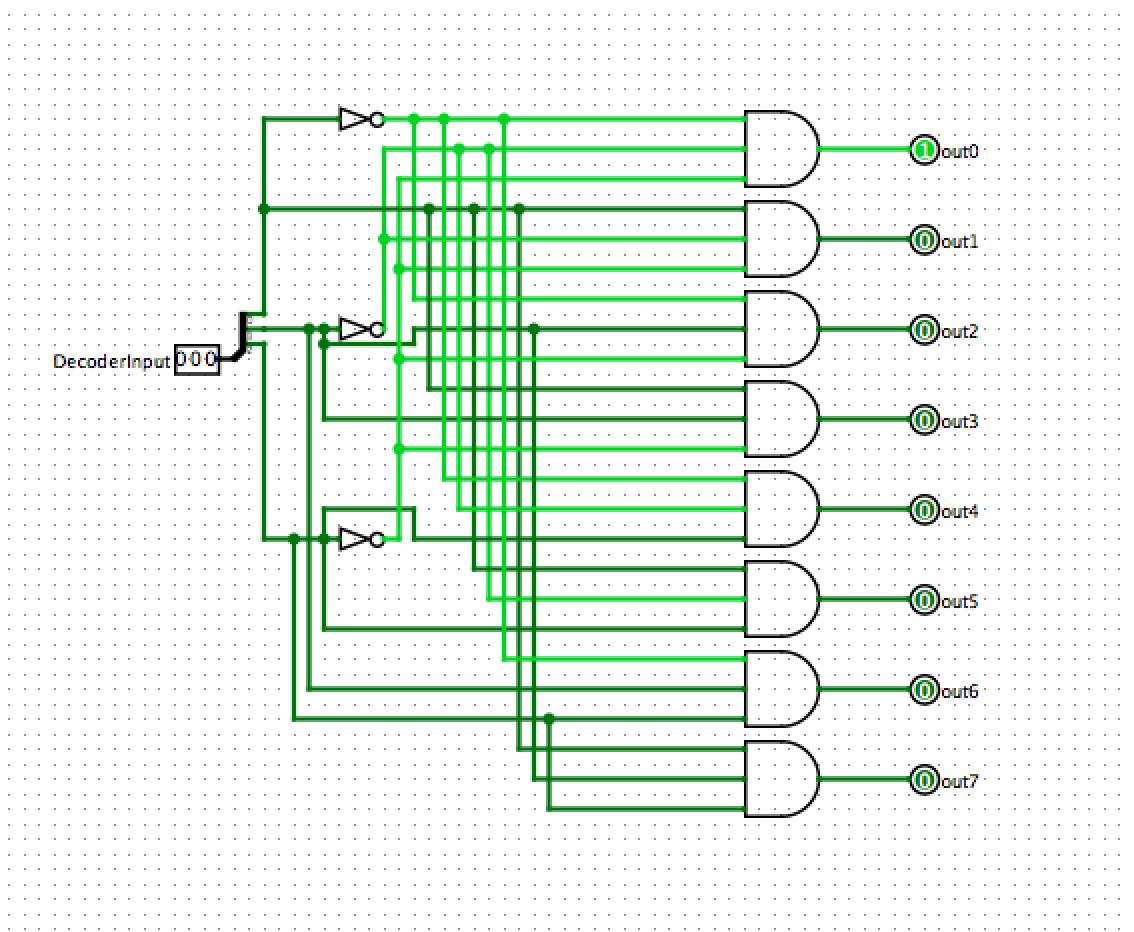
\includegraphics[scale=0.5]{decoder}
			\caption{Decoder Implementation}
		\end{center}
	\end{figure}
	It is just a decoder...nothing fancy about it.
	\clearpage
	\section{Shifter}
	\begin{figure}[H]
		\begin{center}
			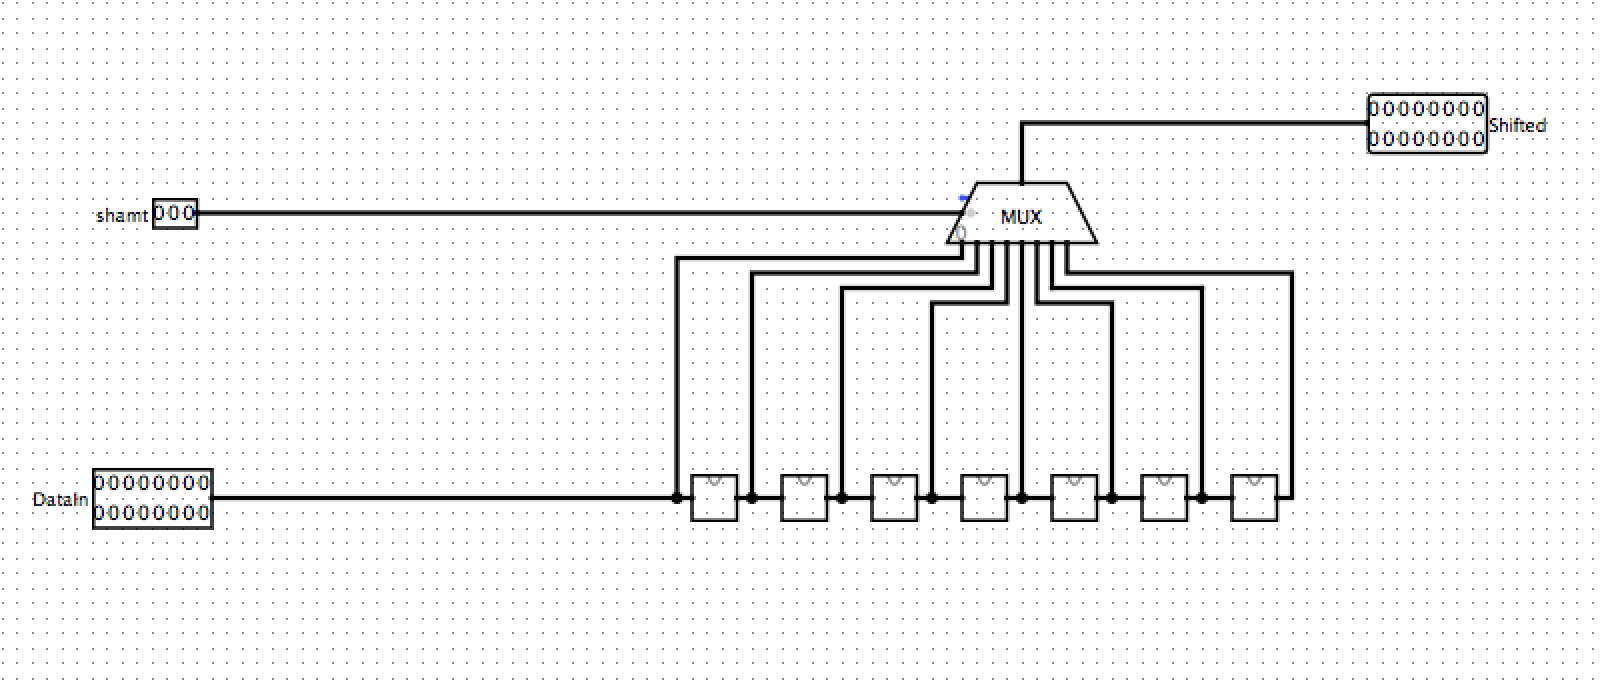
\includegraphics[scale=0.5]{shifter}
			\caption{Shifter Implementation}
		\end{center}
	\end{figure}
	Both the left and right shifters are implemented by connecting a series of 1-bit shifters, and use a multiplexer to choose the correct output. It has two inputs labeled as shamt and DataIn. shamt gives the number of bits shifted and DataIn inputs the number to be shifted. 
	\clearpage
	\section{Control}
	\begin{figure}[H]
		\begin{center}
			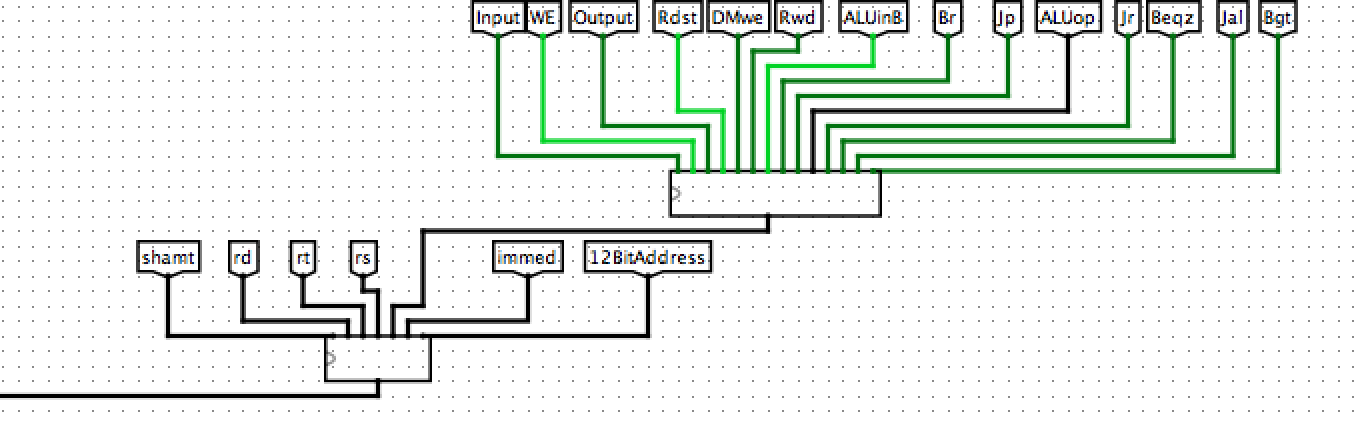
\includegraphics[scale=0.5]{control}
			\caption{Control Implementation}
		\end{center}
	\end{figure}
	The control logic is implemented using two layers. The first layer extracts the necessary bits such as Rs, Rt and opcode values. The second layer has a single input opcode, and translate the opcode into corresponding control signal outputs. 
\end{document}